\documentclass[12pt]{article}
\usepackage[utf8]{inputenc}
\usepackage[T1]{fontenc}
\usepackage{indentfirst}
\usepackage{amsmath}
\usepackage{amssymb}
\usepackage{natbib}
\usepackage{graphicx}
\usepackage{float}
\usepackage[a4paper, margin = 2 cm]{geometry}
\usepackage{fancyhdr}
\usepackage{wrapfig}
\usepackage{hyperref}
\usepackage{mathtools}

\title{Algorytmika praca domowa 2}
\author{Dominik Wawszczak}
\date{2024-04-22}

\begin{document}
    \setlength{\parindent}{0 cm}
    
    Dominik Wawszczak \hfill Algorytmika
    
    numer indeksu: 440014 \hfill praca domowa 2
    
    numer grupy: 1
    
    \bigskip
    \hrule
    \bigskip
    
    Wszystkie porównania były uruchamiane na laptopie z procesorem Intel(R)
    Core(TM) i5-7300HQ CPU @ 2.50GHz, stąd długie czasy działania. Na
    komputerze stacjonarnym ze znacznie mocniejszym procesorem niestety nie
    udało mi się aktywować licencji na GUROBI w WSLu.
    
    \begin{itemize}
        \item[a)] Metodę \texttt{HK} będącą implementacją algorytmu
                  Hopcrofta-Karpa można znaleźć w pliku
                  \texttt{dw440014-assignment2.ipynb}.
        \item[b)] Metody \texttt{LPcbc} oraz \texttt{LPgur} również znajdują
                  się w tym pliku.
        \item[c)] Poniżej znajduje się wykres będący porównaniem działania
                  metod na gęstych losowych grafach o \(n = 300\)
                  wierzchołkach.
                  \begin{center}
                      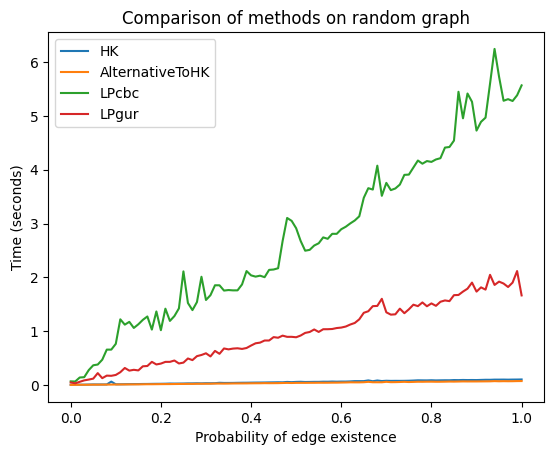
\includegraphics[scale = 0.8]{image_01.png}
                  \end{center}
        \item[d)] Przykładem takiego grafu jest \(k\) rozłącznych ścieżek o
                  długościach kolejno \(1, 3, \ldots, 2k - 1\), dla największego
                  \(k\) spełniającego \(\binom{k + 1}{2} \leqslant n\), czyli
                  dla \(k\) rzędu \(\sqrt{n}\). Jeżeli ponumerujemy wierzchołki
                  w odpowiedniej kolejności, to po pierwszej iteracji algorytmu
                  każda ze wspomnianych ścieżek będzie ścieżką powiększającą.
                  Ścieżki te mają parami różne długości, zatem każda z nich
                  zostanie znaleziona w innej iteracji, skąd wnioskujemy, że
                  algorytm wykona ich \(O \left( \sqrt{n} \right)\).
    \end{itemize}
    
    \newpage
    
    \begin{itemize}
        \item[e)] Ze względu na długi czas działania algorytmu na instancjach z
                  podpunktu d), zdecydowałem się przetestować metody dla \(n\)
                  do \(50\,000\). Wyniki prezentują się następująco:
                  \begin{center}
                      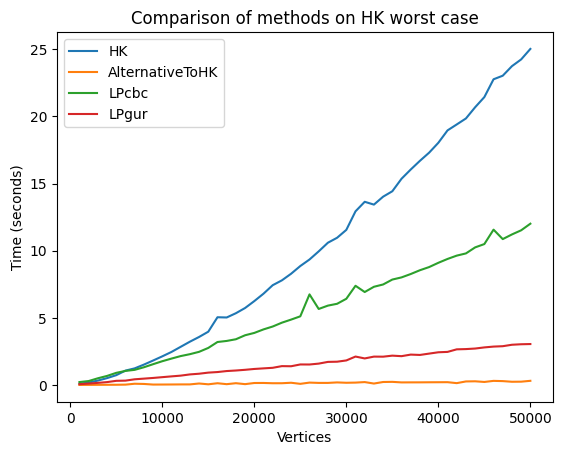
\includegraphics[scale = 0.8]{image_02.png}
                  \end{center}
        \item[f)] Zaproponowaną przeze mnie alternatywą, której implementację
                  można znaleźć w metodzie \texttt{AlternativeToHK}, jest
                  algorytm znany pod nazwą \textit{Turbo matching}, głównie
                  wśród uczestników konkursów typu OI czy ICPC. Nie znam jego
                  złożoności, ale jest bardzo szybki w praktyce i prosty w
                  implementacji -- stąd jego popularność na tego typu
                  konkursach. Nie znam również trudnego przykładu dla tego
                  algorytmu, choć słyszy się legendy o pewnych ,,rosyjskich
                  testach'', na których podobno działa bardzo wolno.
        \item[g)] Dodatkowo przetestowałem wszystkie metody na grafach rzadkich
                  (każdemu wierzchołkowi losujemy sąsiada). Poniżej znajduje
                  się rezultat porównania.
                  \begin{center}
                      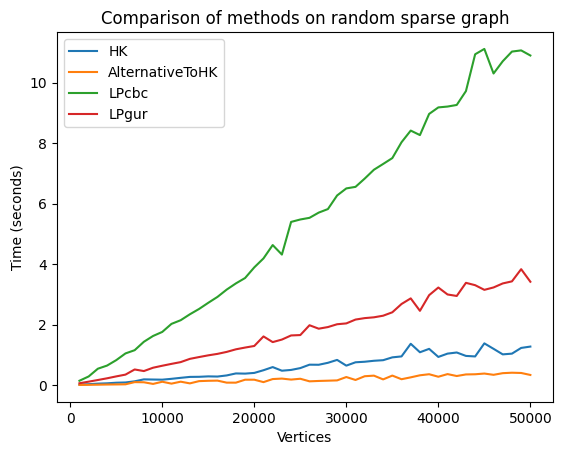
\includegraphics[scale = 0.8]{image_03.png}
                  \end{center}
    \end{itemize}
\end{document}
